\documentclass{article}
\usepackage[UTF8]{ctex}
\usepackage{amsmath}
\usepackage{graphicx}
\usepackage{cite}
\usepackage{subfigure}

\title{龙格-库塔方法与亚当姆斯方法相结合求解微分方程}
\author{21级计算机科学与技术\ 陈岳阳}
\date{\today}

\begin{document}
\maketitle
\tableofcontents

\section{龙格-库塔方法}
  \subsection{龙格-库塔方法的设计思想}
根据微分中值定理,在区间[$x_n, x_{n+1}$]上,存在一点$\eta$使得:
$$
\frac{y(x_{n+1})-y(x_n)}{h}=y'(\eta)
$$

	又已知y'=f,称$K^*=f(\eta, y(\eta))$为[$x_n, x_n+1$]上的平均斜率。只要对平均斜率提供一种算法即可。根据选取的用于计算平均斜率的点数不同,龙格-库塔方法可以达到的截断误差精度也不同。由于推导过程较为繁琐,且结果中的待定参数可以选用不同值,实验仅介绍四阶经典龙格-库塔方法。
    
	\subsection{四阶经典格式龙格-库塔方法}
	经过非常复杂的数学演算,可以导出具有四阶精度的四阶龙格-库塔格式。经典格式是比较常用的一种:
$$
\begin{aligned}
&y_{n+1}=y_n+\frac{h}{6}(K_1+2K_2+2K_3+K_4)\\
&K_1=f(x_n, y_n)\\
&K_2=f(x_{n+\frac{1}{2}, y_n+\frac{h}{2}K_1})\\
&K_3=f(x_{n+\frac{1}{2}, y_n+\frac{h}{2}K_2})\\
&K_4=f(x_{n+1},y_n+hK_3)\\
\end{aligned}
$$

\section{亚当姆斯方法}
	前述的龙格-库塔方法是一类重要算法,但它在每次计算下一点的值时,都需要先对几个点上的函数值进行预报,计算量比较大。考虑到或许可以利用之前计算出的斜率,亚当姆斯方法合乎逻辑的出现了。
  \subsection{亚当姆斯格式的设计}
	这里介绍二阶亚当姆斯格式的设计思路,更高阶的亚当姆斯格式可以通过类似的思想得出。实验中使用了四阶亚当姆斯格式。

	计算$y_{n+1}$时,希望使用$y'_{n-1}$和$y'_n$来计算$[y_n, y_{n+1}]$的平均斜率,有如下计算式:
$$
\begin{aligned}
&y_{n+1}=y_n+h[(1-\lambda)y'_n+\lambda y'_{n-1}\\
&y'_n=f(x_n, y_n)\\
&y'_{n-1}=f(x_{n-1}, y_{n-1})
\end{aligned}
$$
假设$y_n$和$y_{n-1}$都是精确值,若使$y_{n+1}$有二阶精度,将$y'_{n-1}$在点$x_n$处展开,比对系数,可知$\lambda=-\frac{1}{2}$,得到显式亚当姆斯格式:
$$
y_{n+1}=y_n+\frac{h}{2}(3y'_n-y'_{n-1})
$$

如果选取的两个点为$x_{n+1}$和$x_n$,则可以类似得到隐式亚当姆斯格式。

类似地,可以导出四阶显式亚当姆斯格式和四阶隐式亚当姆斯格式:
$$
\begin{aligned}
&y_{n+1}=y_n+\frac{h}{24}(55y'_n-59y'_{n-1}+37y'_{n-2}-9y'_{n-3})\\
&y_{n+1}=y_n+\frac{h}{24}(9y'_{n+1}+19y'_n-5y'_{n-1}+y'_{n-2})\\
\end{aligned}
$$

	\subsection{亚当姆斯预报-校正系统}
先使用显式亚当姆斯格式对$y_{n+1}$进行预报,然后使用预报值进行隐式亚当姆斯格式,计算出$y_{n+1}$的真实值。

由于四阶亚当姆斯格式需要前四个点的导数值,需要先使用四阶经典龙格-库塔格式计算三个点的导数值,然后启动亚当姆斯算法。
\begin{figure}[tbp]
\centering
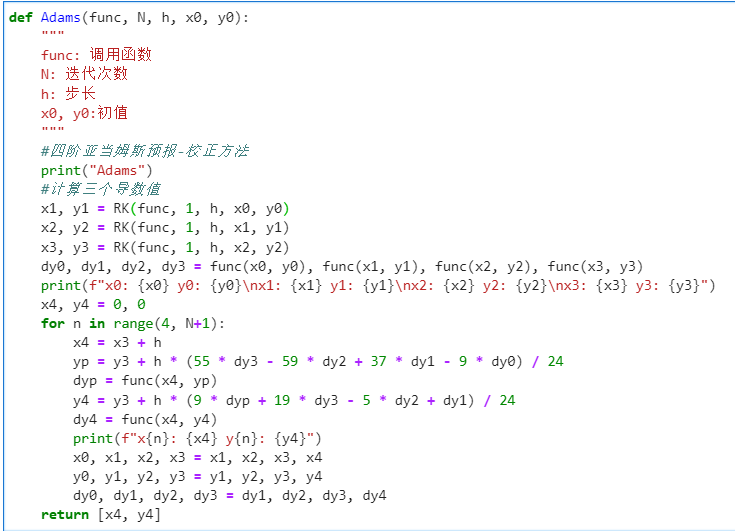
\includegraphics[width=6cm,height=4.8cm]{adams.png}
\caption{亚当姆斯预报校正}
\end{figure}
\newpage
\section{实验代码及解决问题}
实验代码及详细注释在附件“陈岳阳-第三章实验.md”中,使用四阶经典格式龙格库塔方法和四阶亚当姆斯预报-校正算法计算了书P98.例1和P124.12,并与精确解或书上给出结果进行比较。此处仅提供两张结果图,详细代码请阅读附件。
\begin{figure}
	\centering
	\subfigure[f1测试结果]{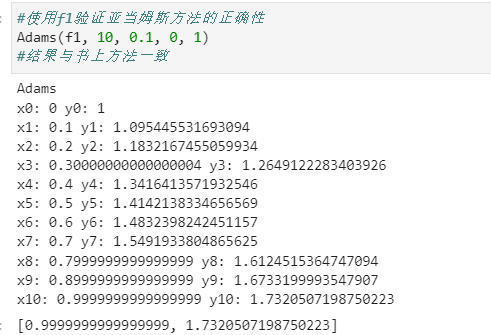
\includegraphics[width=6cm]{实验结果1.png}}
	\subfigure[f2测试结果]{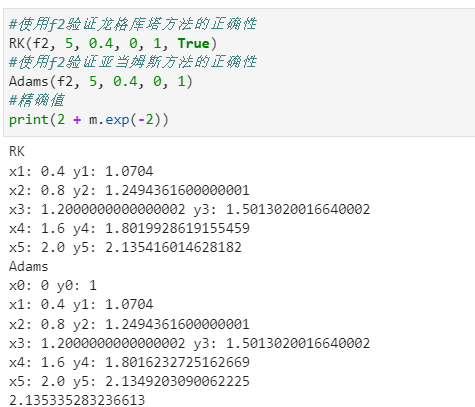
\includegraphics[width=6cm]{实验结果2.png}}
	\caption{实验结果}
\end{figure}
\end{document}